\section{Method}

\subsection{The task and partial goals}

The final goal, or task, to accomplish was pushing a cube from and to some
arbitrary positions in the workspace of the robot. The task was researched
using a reinforcement learning approach, only specifying the wanted behavior by
defining a reward function $f(s, a, s') \in \mathbb{R}$, where $s, a, s'$ is
the state, action, and successor state. The state here includes the robot and
cube state along with the goal. First-order Markov property is assumed together
with assuming the state as observable, formulating the problem as a Markov
Decision Process (MDP).

An iterative approach was taken in order to solve the
task, starting by solving simpler tasks before increasing the complexity. This
way algorithms are sanity checked in a natural fashion and making limitations
of model formulations clearer as complexity is added. The first task was to
investigate appending arbitrary goals to the state for a reaching task with a
simulated agent and environment. This was later extended to being trained on
data from distributed real robotic systems. Pushing tasks were then attempted
in simulation followed by evaluating trained policies on real robots. As a
second part to this thesis, pose estimation from camera was researched with the
goal to relax the assumption of a fixed position camera or known offset to the
camera. This was also done in an iterative fashion starting with a fixed
position camera and then using simulations to investigate neural network
capabilities given perfect features. Finally, results regarding pose estimation
were evaluated on the real robotic systems replacing pose estimates from other
sensors.

\subsection{Robotic environment}
\label{sec:robo_env}

Low cost robotic arms (uArm Metal) were used along with a dedicated computer,
and a \textit{LIght Detection And Range}-device (LIDAR) for pose estimation of
the cube. For pose estimation from camera, an RGB-camera with an optional
RGB-aligned depth channel was used. A workspace for the entire setup was
defined to be $x \in [-0.1, 0.1]$, $y \in [0.1, 0.3]$ (meters), both for the
reaching and pushing task. The coordinate frame used is shown in figure
\ref{fig:workspace_lidar_place} (top left), along with the placement of the
LIDAR and camera (top right).

\begin{figure}[h]
    \centering
    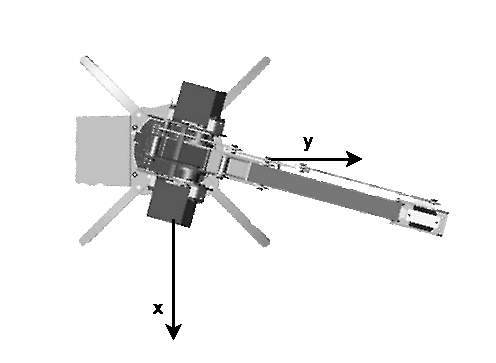
\includegraphics[width=0.50 \textwidth]{res/uarm_coordinates.pdf}
    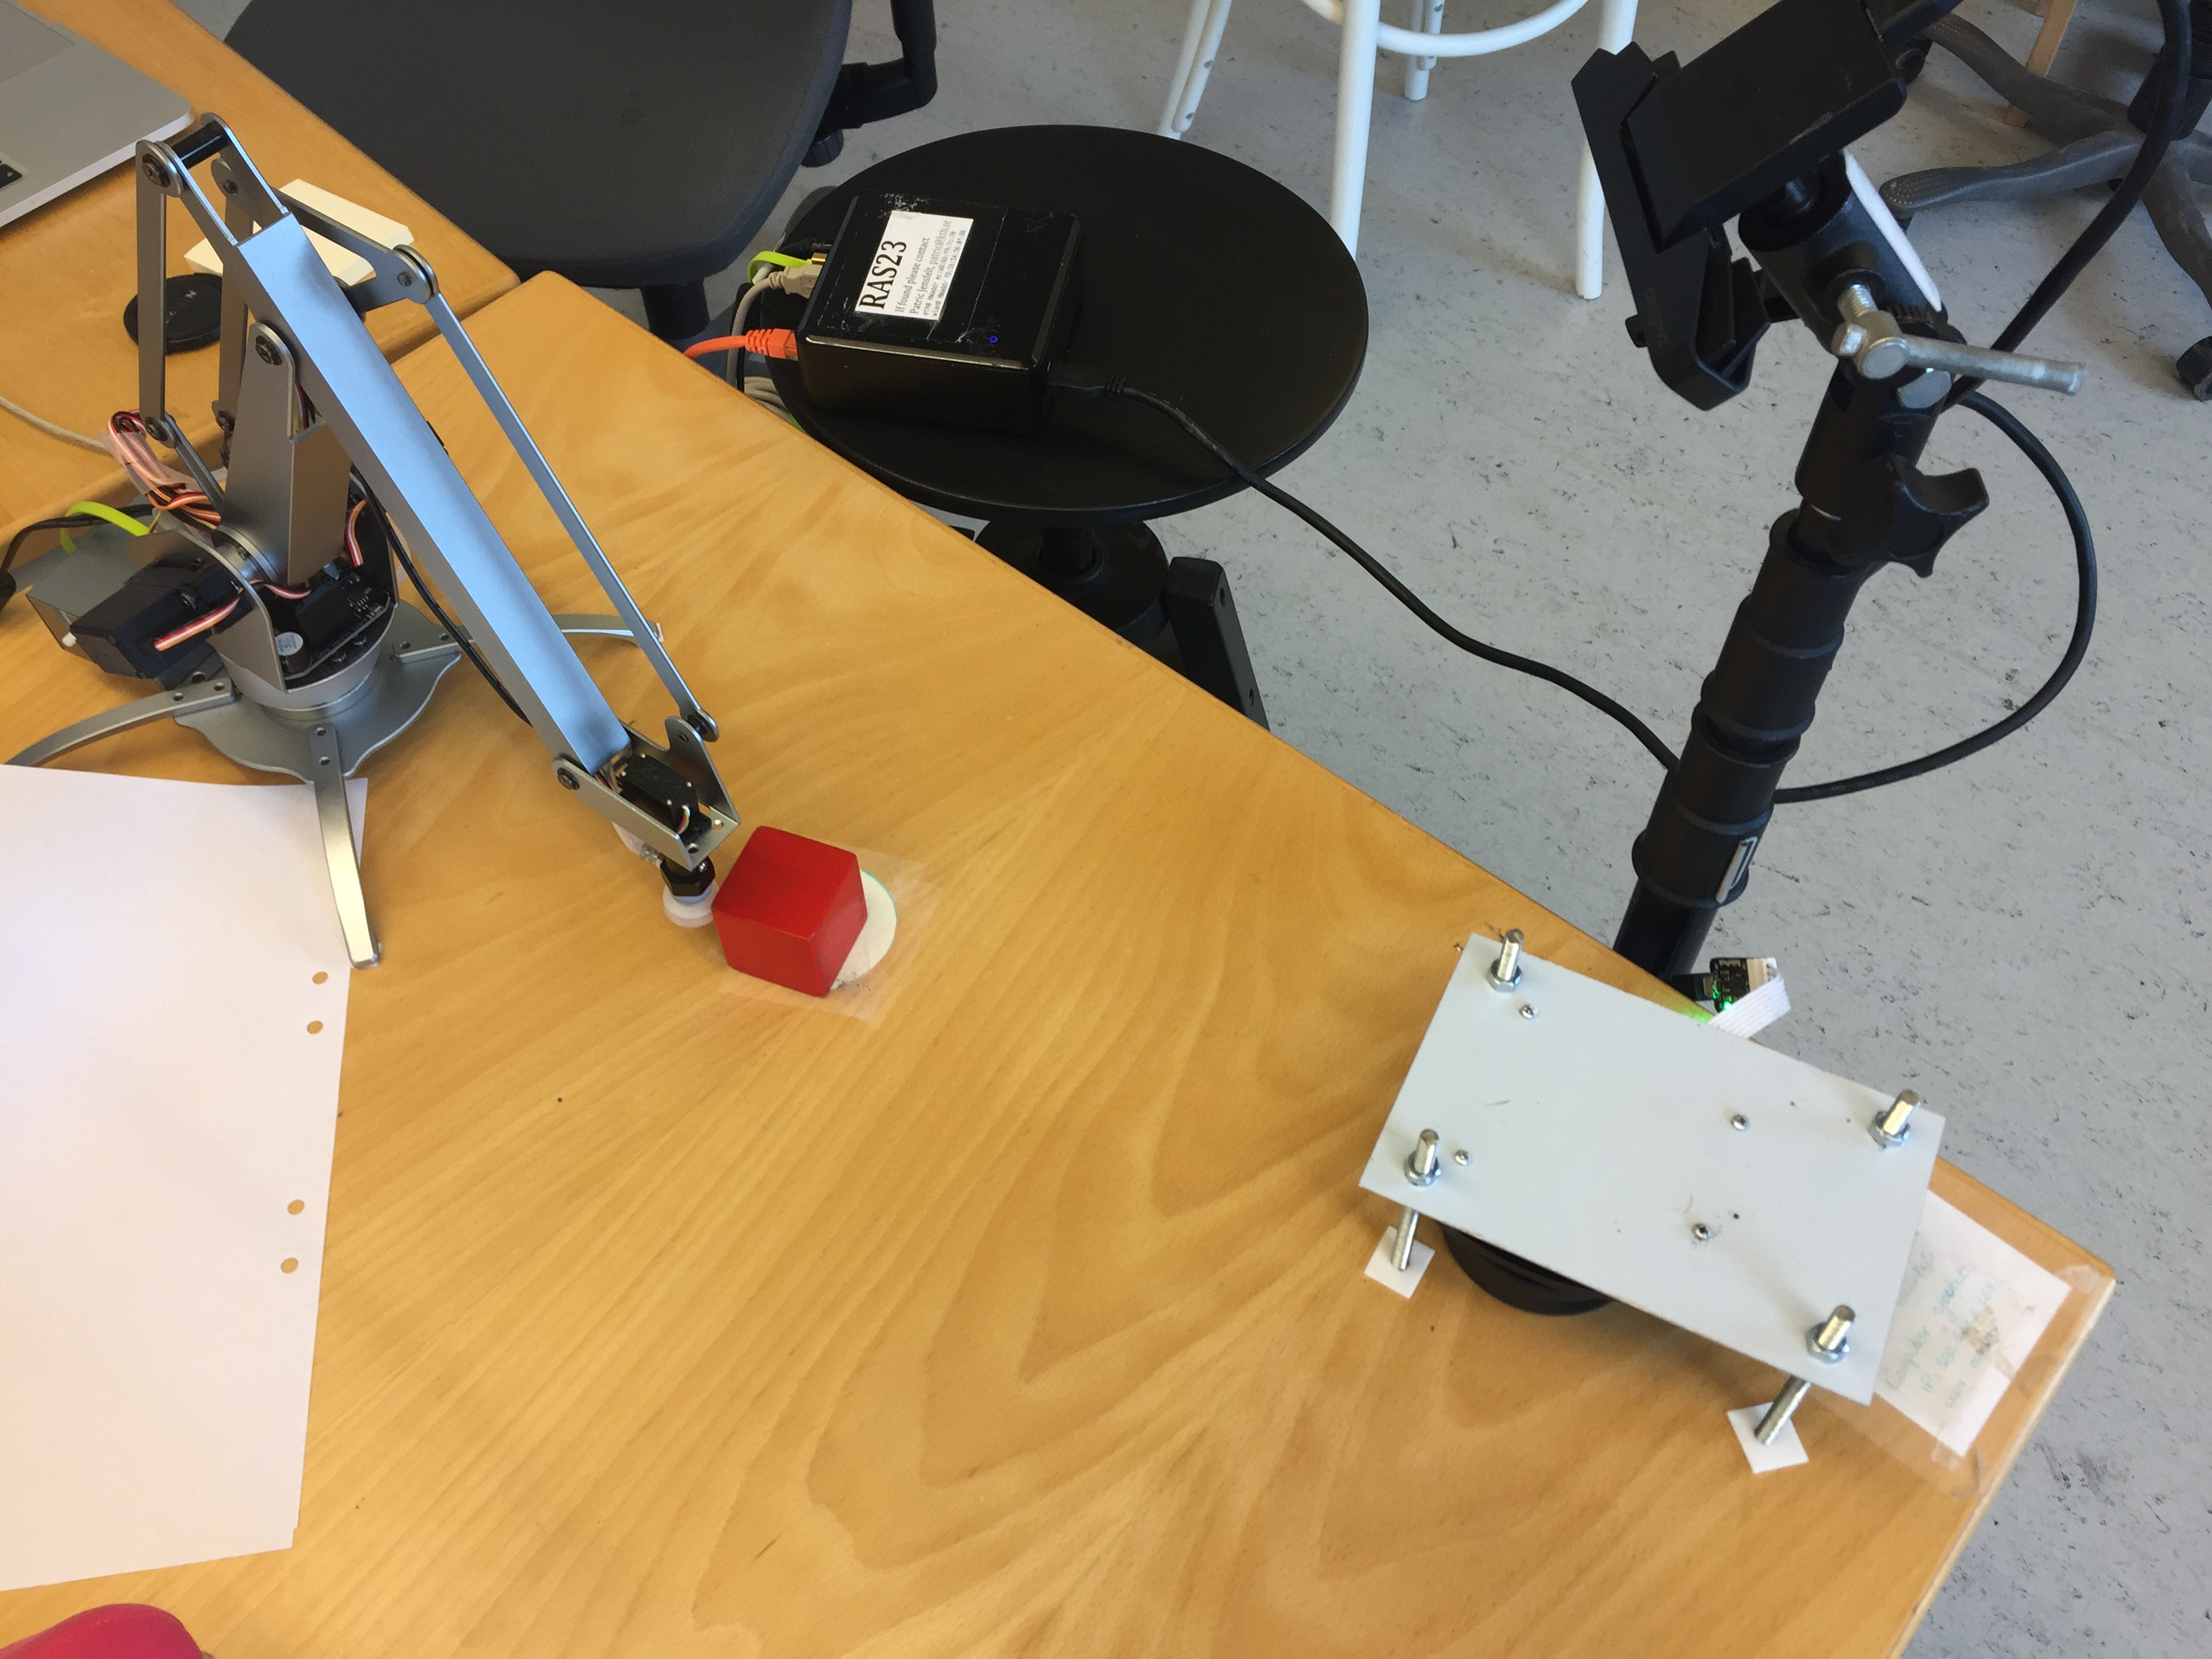
\includegraphics[width=0.49 \textwidth]{res/camera_placement_fixed.jpg}
    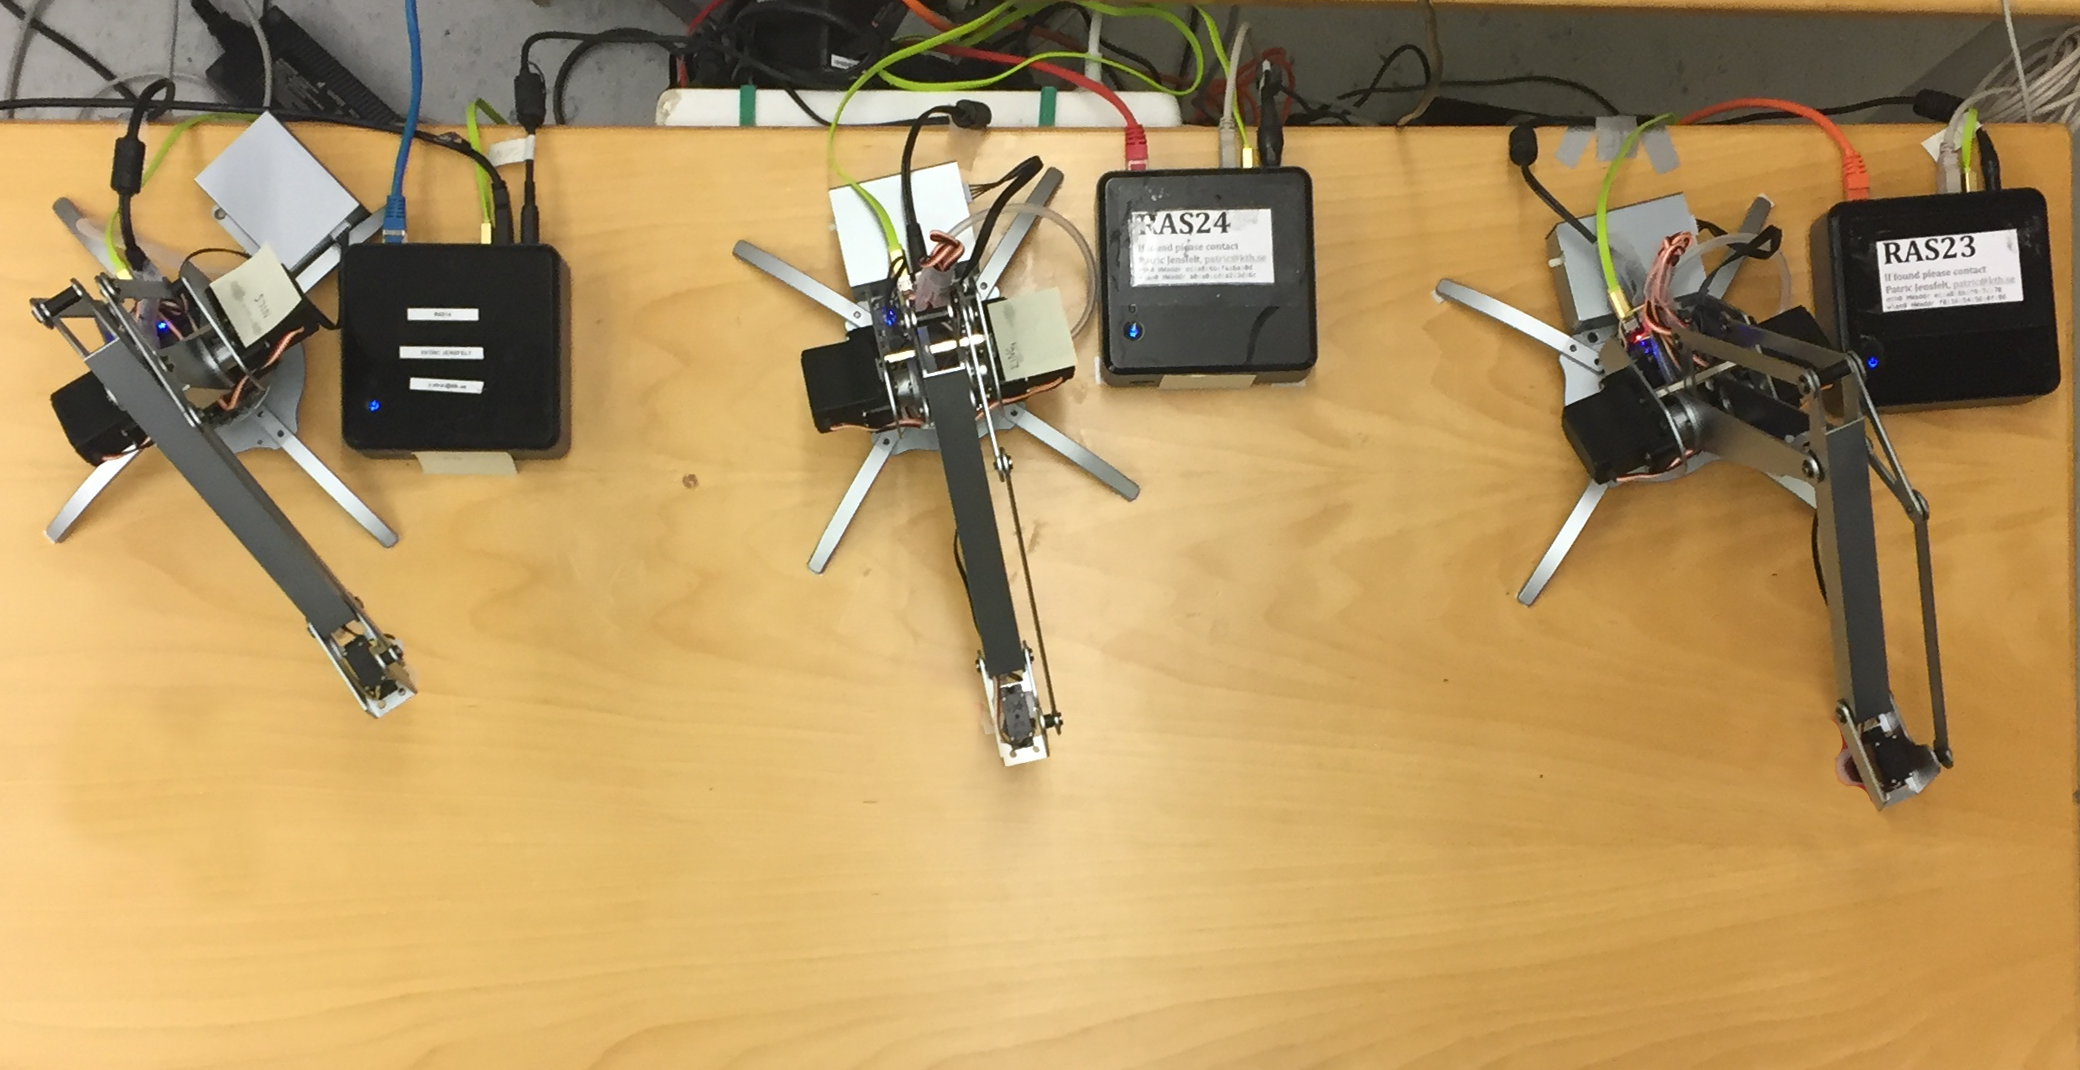
\includegraphics[width=1.00 \textwidth]{res/uarm_moving_setup.png}

    \caption{Top left: Coordinate frame used for the robot. Top right:
    Placement of the LIDAR, seen attached to a gray housing in the bottom right
    corner. The housing was built in order to mount the LIDAR such that it only
    registers reflecting light from the cube. The fixed camera position for
    cube pose estimation can also be seen in the top right corner of this picture.
    Bottom: For distributing data collection, several setups, each with a
    dedicated computer, was used.}

    \label{fig:workspace_lidar_place}

\end{figure}

The arms were in this thesis controlled by commanding servo angles, with an
implemented controller on top that could command the end-effector to some
cartesian coordinates. The arms have 4 degrees of freedom, but only three were
used in this thesis, ignoring the end-effector rotation servo. The arms were
shipped with controllers and forward/inverse kinematics but were not reliable,
therefore new derivations of the kinematics were done along with a new
controller implementation.

\subsubsection{Inverse kinematics derivation}

Definition of landmarks and distances can be seen in figure
\ref{fig:uarm_landmarks}. We are given the coordinates of the point $D$ and
want to find to angles $\alpha$, $\beta$, and $\theta$.

\begin{figure}[!ht]
    \centering
    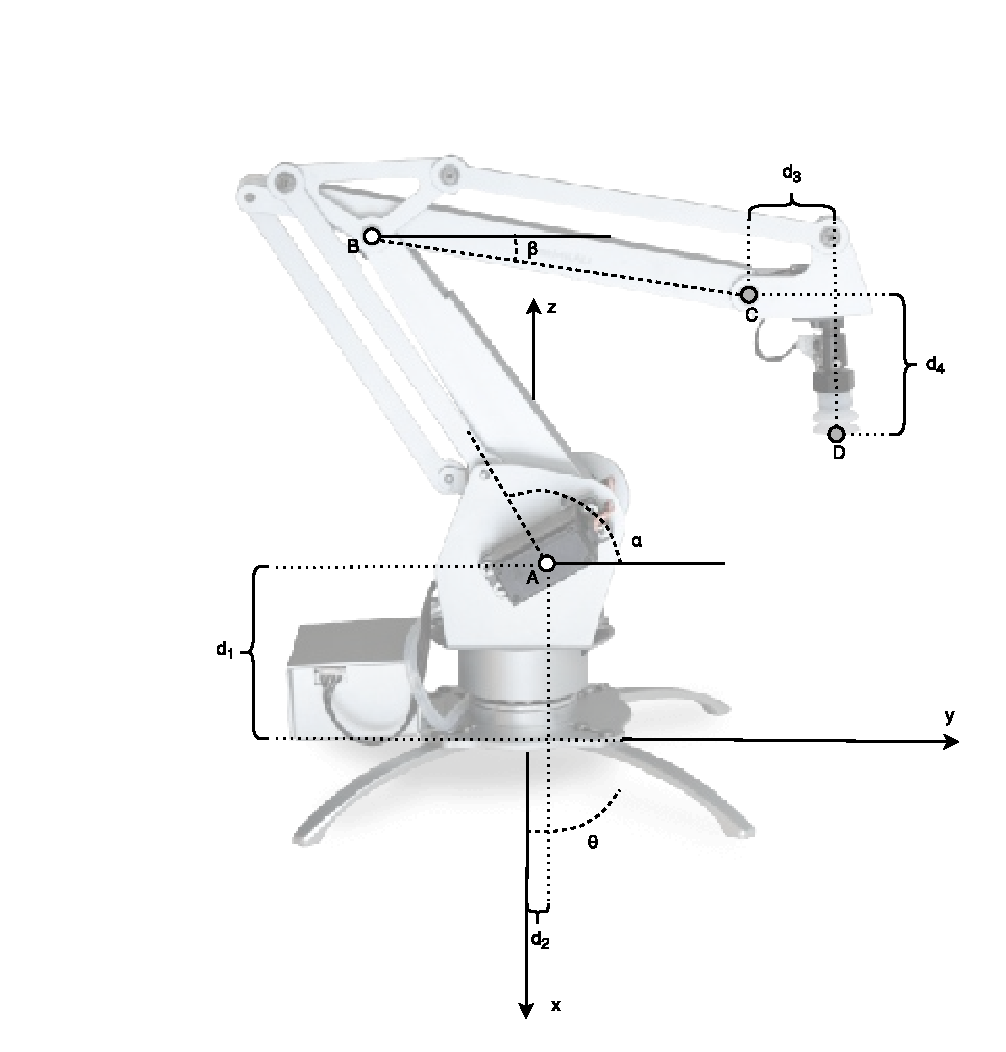
\includegraphics[width=0.80 \textwidth]{res/inverse_kinematics.pdf}

    \caption{Notation for landmarks used in derivation of inverse kinematics. A
    simplified problem is to consider the angles of the triangle $ABC$.}

    \label{fig:uarm_landmarks}

\end{figure}

The angle $\theta$ of the bottom servo that rotates the arm around the z-axis
is first simply found by:

\begin{equation}
    \theta = \text{arctan2}(y, x)
\end{equation}

The problem can then be simplified by considering the 2D problem where the
origin is placed at $A$, consider $C$ instead of $D$ which is easily found, in
the 2D plane defined by the points $A, B, C$. Denote the coordinates of $C$ in
this new frame as:

\begin{equation}
    r = \sqrt{x^2 + y^2} - d_2 - d_3
\end{equation}

\begin{equation}
    h = z - d_1 - d_4
\end{equation}

Distances $d_{AB}$ and $d_{BC}$ are known constants, $d_{AC}$ is simply
$\sqrt{r^2 + h^2}$. Define the part of the $\alpha$ angle pointing towards
$C$ from $A$ as $\gamma$. This is found by:

\begin{equation}
    \gamma = \text{arctan2}(h, r)
\end{equation}

All sides of the triangle $ABC$ are known, so the angles are found by the rule (applied in the same fashion to all angles):

\begin{equation}
    \cos(BAC) = \frac{d_{AB}^2 + d_{AC}^2 - d_{BC}^2}{2 d_{AB} d_{AC}}
\end{equation}

The angle $\alpha$ is found by:

\begin{equation}
    \alpha = BAC + \gamma
\end{equation}

The angle between the vertical line going down from $A$ and $AB$ is $\alpha - \frac{\pi}{2}$
which implies:

\begin{equation}
    \beta = \frac{\pi}{2} - ABC - (\alpha - \frac{\pi}{2}) = \pi - ABC - \alpha
\end{equation}

\subsection{Simulated environment}

A simple 2D environment was implemented with a circular pushable object, and a
point-like manipulator. Actions was sent to the environment as relative
movement of the manipulator. The environment does not take friction into
account, only moving the pushable object the minimum distance so that the
manipulator never exists within the object boundaries. Positions of goal,
manipulator, and object could be sampled according to different sampling
strategies, in the full problem each position is sampled uniformly within the
workspace. Samples of this environment is shown in figure
\ref{fig:env_sim_samples}. After each interaction, the environment returns
successor state and reward. For reaching tasks in simulation, the pushable
object is simply ignored.

\begin{figure}[!ht]
    \centering
    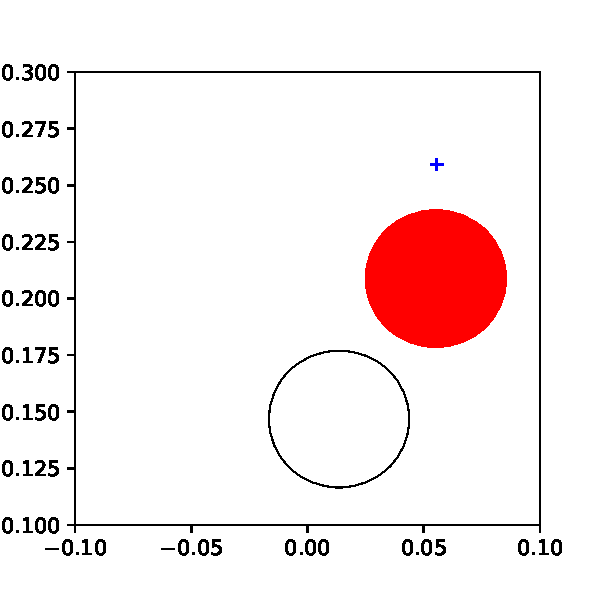
\includegraphics[width=0.3\textwidth]{res/env_sim1.pdf}
    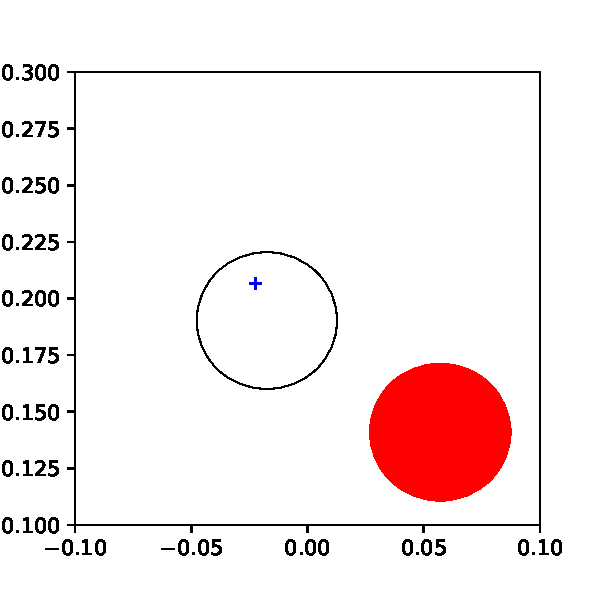
\includegraphics[width=0.3\textwidth]{res/env_sim2.pdf}
    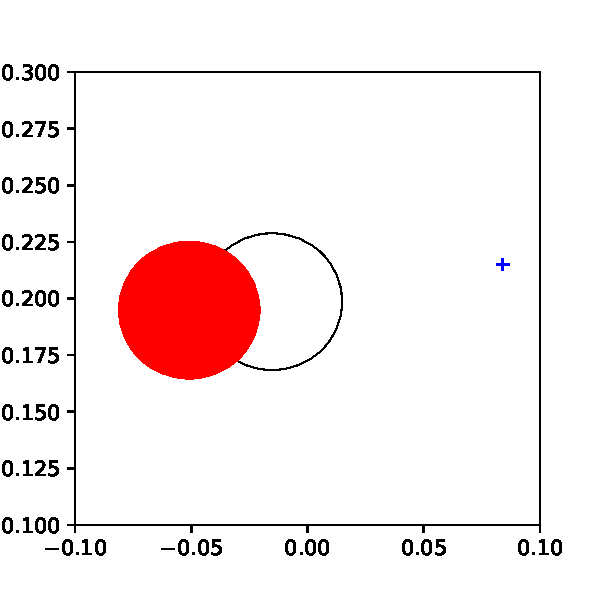
\includegraphics[width=0.3\textwidth]{res/env_sim3.pdf}

    \caption{The simulated environment for pushing, the cross represents the
    robot end-effector, red circle the pushable object, and the black/white
    circle the goal position.}

    \label{fig:env_sim_samples}
\end{figure}

\subsection{Estimating the cube position using LIDAR}

A LIDAR was used to estimate the position of the cube. These estimates were
both used as ground truth for training pose estimation neural networks, and
used as a part of the state for the reinforcement learning algorithms. The
LIDAR gives $360$ distance measurements at approximately evenly spaced angles,
with the angles having some variation from sweep to sweep. By sweep here is
meant a new set of 360 measurements from a full rotation of the laser. Sweeps
are returned at $10$ Hz. Only scans inside the defined workspace (section
\ref{sec:robo_env}) were considered for pose estimation of the cube. Only the
cube is assumed to reflect light from the LIDAR, the end-effector of the robot
was placed at a z-coordinate such that it is above the plane of the
LIDAR-scans.

To estimate the cube pose, the Hough-transform was used \cite{duda1972use}.
This algorithm takes as input a 2D matrix and returns scalar values for a set
of angles and distances $\lbrace \theta_1, ..., \theta_M\rbrace \times \lbrace
d_1, ..., d_N \rbrace$ each defining a line in the plane, see figure
\ref{fig:hough}. A large scalar for some $\theta_i$ and $d_i$ means that the
matrix entries along the coordinates specified by these parameters have higher
values, i.e. pixels form a line along the parameterized line.

\begin{figure}[h]
    \centering
    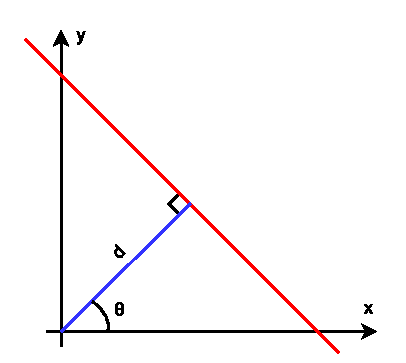
\includegraphics[width=0.40\textwidth]{res/hough.pdf}

    \caption{The Hough transform returns scalar values for a set of lines each
    parameterized by some $\theta$ and $d$. In this figure the red line is
    parameterized by the angle $\theta$ and distance $d$.}

    \label{fig:hough}
\end{figure}

The angles with corresponding distance measures from the LIDAR are converted to
cartesian space and plotted onto a matrix (Hough transform input), an example
is shown in figure \ref{fig:hough_example} where the black pixels correspond to
LIDAR scans. After applying the transform on this image, the line with the
highest corresponding scalar value is chosen, in figure \ref{fig:hough_example}
shown as the red line. One of the cube's sides can then be estimated using this
line, limited by the outermost scans lying approximately on this line, see red
dots in figure \ref{fig:hough_example}. The center of the cube, which is
$4\times 4\times 4$ cm, is then estimated by adding the orthogonal vector of
length $2$ cm from the center of the estimated cube side (shown as blue dot).
Only the center of the cube was used for the experiments, although the full
pose of the cube is easily inferred from the found line.

\begin{figure}[h]
    \centering
    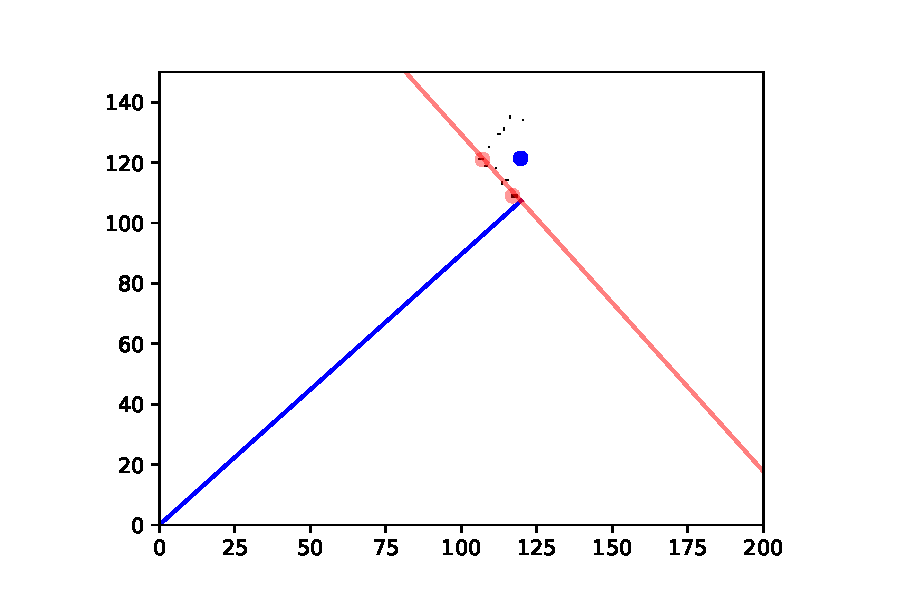
\includegraphics[width=0.60\textwidth]{res/hough_example.pdf}

    \caption{LIDAR scans are plotted onto a binary matrix. The parameters with
    the maximum output from the Hough transform corresponds to the red line.
    The side of the cube is estimated by taking the outermost scans
    approximately lying on this line. The center of the cube is then found by
    adding an orthogonal vector from the center of this side with length
    corresponding to half of the cube size.}

    \label{fig:hough_example}
\end{figure}

The scans from the LIDAR showed variation between sweeps resulting in
variations in the pose estimates. This can be seen in figure
\ref{fig:lidar_noise}. The noise being relatively large imposes difficulties in
training policies using this data, and also for training neural network pose
estimators using LIDAR estimates as ground truth. Averaging estimates is one
solution to lowering errors but implies slower updates of the pose estimation.

\begin{figure}[h]
    \centering
    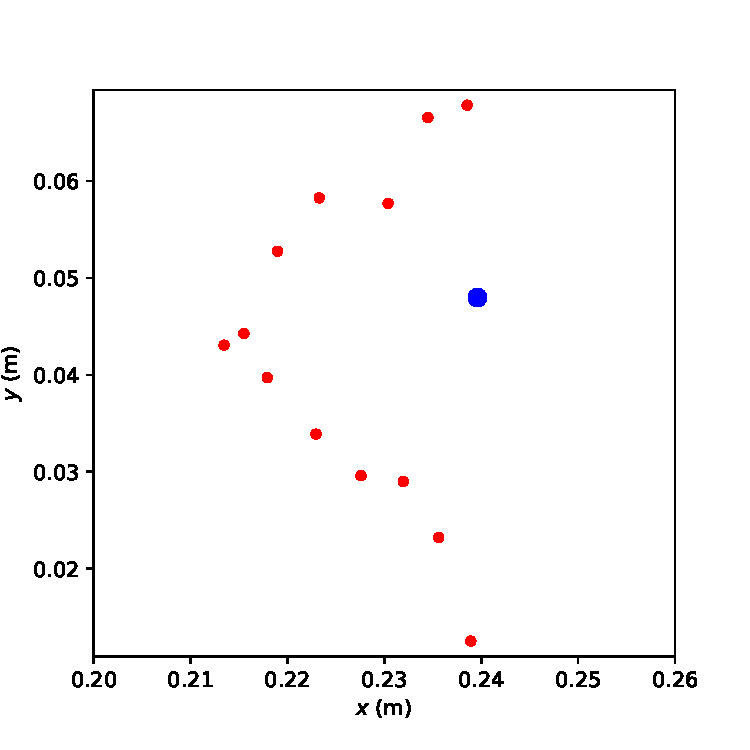
\includegraphics[width=0.49\textwidth]{res/cube_pose_lidar_one_scan.pdf}
    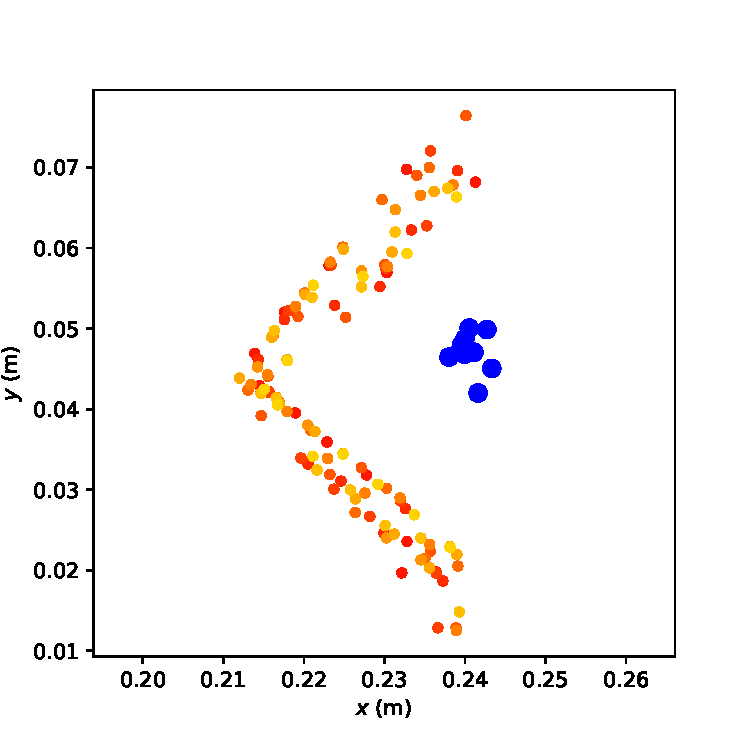
\includegraphics[width=0.49\textwidth]{res/cube_pose_lidar_variance.pdf}

    \caption{LIDAR scans (red) on a cube with the corresponding position
    estimate (blue). To the left one single sweep with the LIDAR clearly
    showing noisy measurements. To the right, plotting consecutive scans for
    the same cube position along with cube pose estimates shows noisy
    measurements and also noisy pose estimates of the cube. The different
    colors of the scans to the right represent different sweeps and show that
    the noise does not have a bias that is unique to the current sweep.}

    \label{fig:lidar_noise}
\end{figure}

\subsection{Software and libraries}

For high-level computational graphs, Keras \cite{chollet2015keras} was used.
For lower-level extensions not supported by Keras, Theano was used
\cite{theano2016theano}. For image pre-processing, plotting, and overall linear
algebra and mathematical computations, SciPy was used \cite{scipy2016scipy}.
